
% --- Définition ---
\begin{frame}{1. Définition d'une Courbe Elliptique}
\frametitle{Définition d'une Courbe Elliptique}

Une courbe elliptique $E$ est définie par l'équation :
$$y^2 = x^3 + ax + b$$

Pour la cryptographie (ECDSA), nous travaillons sur un \textbf{Corps Fini} $\mathbb{F}_p$ où $p$ est un nombre premier. L'équation devient :
$$y^2 \equiv x^3 + ax + b \pmod{p}$$

\begin{itemize}
    \item \textbf{Les éléments :} L'ensemble des points $(x, y)$ satisfaisant l'équation, plus un point spécial : le \textbf{Point à l'Infini} ($\mathcal{O}$).
    \item \textbf{Non-singularité :} Pour assurer une courbe lisse (pas de points de rebroussement), le discriminant doit être non nul : $\Delta = 4a^3 + 27b^2 \not\equiv 0 \pmod{p}$.
\end{itemize}
\end{frame}

% --- Addition ---
\begin{frame}{2. L'Opération d'Addition ($P + Q$)}
\frametitle{L'Opération d'Addition ($P + Q$)}

    \begin{columns}
        \column{0.5\textwidth}
        L'addition de deux points $P$ et $Q$ sur la courbe donne un troisième point $R$.
\textbf{Géométriquement :}
\begin{enumerate}
    \item Tracer la droite passant par $P$ et $Q$.
    \item Elle coupe la courbe en un 3ème point $R'$.
    \item Le résultat $R$ est le symétrique de $R'$ par rapport à l'axe des abscisses.
\end{enumerate}



\textbf{Élément neutre :}
$$P + \mathcal{O} = P \quad \text{et} \quad P + (-P) = \mathcal{O}$$
où $-P$ est le point $(x, -y)$.

    \column{0.5\textwidth}
    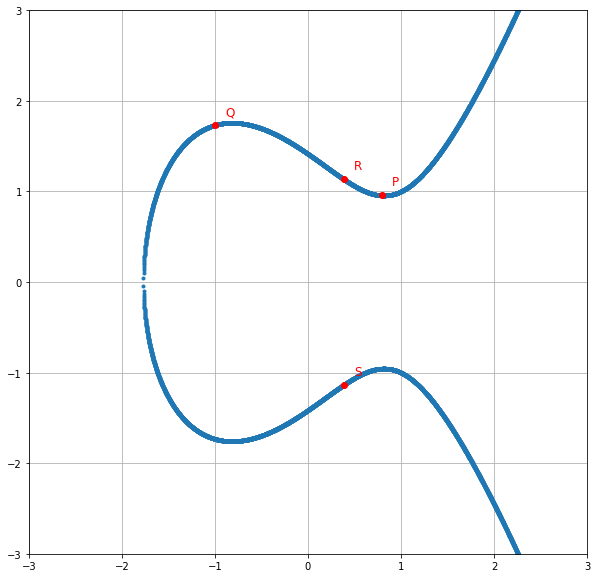
\includegraphics[width=\linewidth]{plot_courbe_elliptique.png}
    \end{columns}


\end{frame}

\begin{frame}{Formules Algébriques de l'Addition}
\frametitle{Implémentation dans $\mathbb{F}_p$}

Soient $P=(x_P, y_P)$ et $Q=(x_Q, y_Q)$. On calcule d'abord la pente $s$ (slope).

\textbf{Cas A : Addition ($P \neq Q$)}
$$s \equiv \frac{y_Q - y_P}{x_Q - x_P} \pmod{p}$$

\textbf{Cas B : Doublement ($P = Q$)}
$$s \equiv \frac{3x_P^2 + a}{2y_P} \pmod{p}$$

\textbf{Résultat $R=(x_R, y_R)$ :}
$$x_R \equiv s^2 - x_P - x_Q \pmod{p}$$
$$y_R \equiv s(x_P - x_R) - y_P \pmod{p}$$
\end{frame}

% --- Multiplication ---
\begin{frame}{3. La Multiplication Scalaire ($k \cdot P$)}
\frametitle{La Multiplication Scalaire ($k \cdot P$)}

La multiplication scalaire consiste à additionner un point $P$ avec lui-même $k$ fois :
$$Q = k \cdot P = \underbrace{P + P + \dots + P}_{k \text{ fois}}$$

\begin{itemize}
    \item \textbf{Facile à calculer :} Grâce à l'algorithme "Double-and-Add" (complexité logarithmique).
    \item \textbf{Difficile à inverser :} Retrouver $k$ à partir de $Q$ et $P$ est le problème du \textbf{Logarithme Discret (ECDLP)}. C'est ce qui sécurise votre clé privée.
\end{itemize}

\begin{block}{Exemple du notebook ($p=41$)}
Clé privée $d=17$, Point $G=(12, 5)$.
Clé publique $Q = 17 \cdot G = (17, 17)$.
\end{block}
\end{frame}

% --- Ordre ---
\begin{frame}{4. L'Ordre de la Courbe et du Point}
\frametitle{L'Ordre de la Courbe et du Point}

\begin{block}{Ordre d'un point $G$}
L'ordre $n$ d'un point $G$ est le plus petit entier positif tel que :
$$n \cdot G = \mathcal{O} \quad (\text{Point à l'infini})$$
\end{block}

\begin{itemize}
    \item Cela signifie qu'après $n$ additions, on "boucle" et on revient à l'élément neutre.
    \item \textbf{Théorème de Hasse :} L'ordre $N$ de la courbe (nombre total de points) est proche de $p$ :
    $$|N - (p+1)| \le 2\sqrt{p}$$
\end{itemize}

\textbf{Application :} Dans le notebook, pour $p=41$, l'ordre du point générateur $G$ trouvé est $n=21$.
\end{frame}

% --- Conclusion ---
\begin{frame}{Conclusion}
\frametitle{Résumé des Opérations}

L'implémentation manuelle de l'ECDSA repose entièrement sur ces briques :

\begin{enumerate}
    \item \textbf{Corps Fini :} Calculs modulo $p$ pour limiter la taille des nombres.
    \item \textbf{Addition :} Combinaison géométrique traduite en formules algébriques.
    \item \textbf{Multiplication :} Série optimisée d'additions et de doublements.
    \item \textbf{Ordre :} Définit la taille de l'espace des clés (sécurité).
\end{enumerate}

Ces opérations mathématiques pures permettent de construire les primitives de \textit{Signature} et de \textit{Vérification}.
\end{frame}
